% %*----------- SLIDE -------------------------------------------------------------
% \begin{frame}[c]{}

%     \centering
%     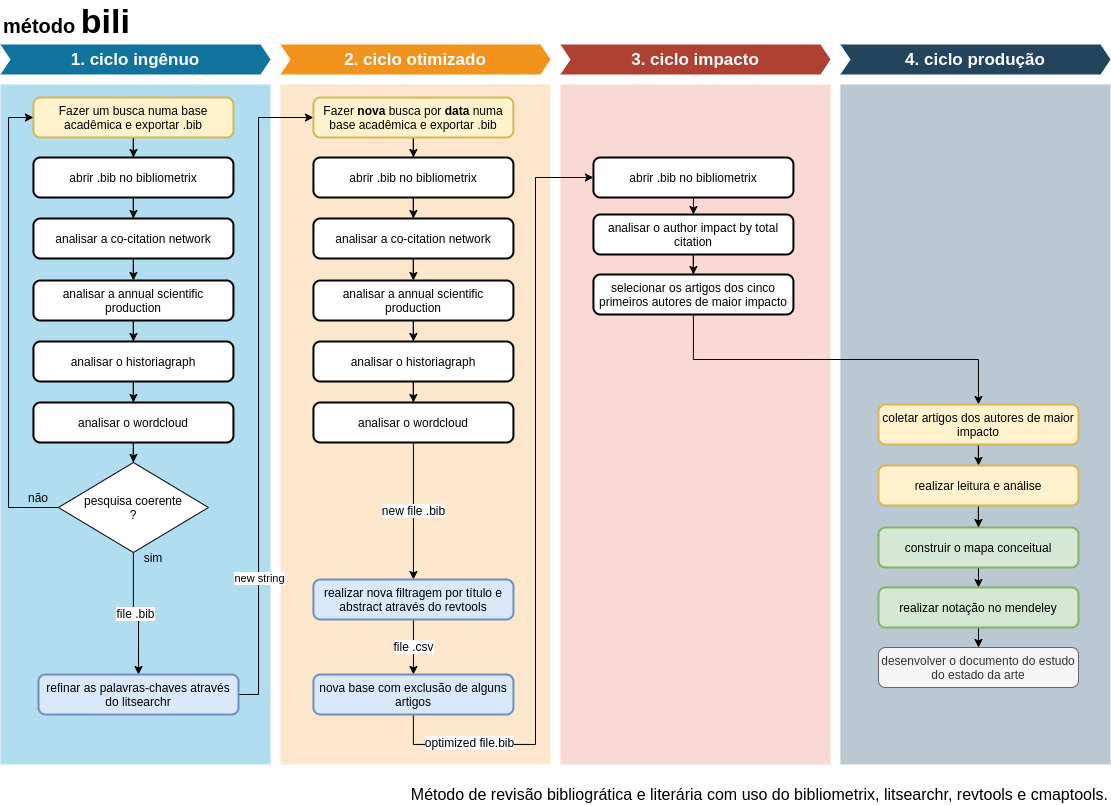
\includegraphics[width=.85\textwidth, trim= 0 30 0 0, clip]{revisão bibliogrática Diagram.png}
    
        
%     % \begin{tikzpicture}[remember picture,overlay]
%     %     \draw[red,very thick] (cmark) circle[x radius=8mm,y radius=4mm]; 
%     % \end{tikzpicture}
% %*----------- notes
%     \note[item]{Notes can help you to remember important information. Turn on the notes option.}
% \end{frame}
% %-
% %*----------- SLIDE -------------------------------------------------------------
% \begin{frame}[t]{O progresso das equipes}
%     Um dos indicadores para o acompanhamento das equipes será o percentual de conclusão geral da equipe.
%     O planejamento das atividades deverá seguir a metodologia aplicada no desenvolvimento de projetos de robótica.
%     \newline
%     %\vspace{0.5cm}
%     \begin{table}[ht!]
%     \centering
%         \caption{PERCENTUAL DE CONCLUSÃO POR EQUIPE}
%         \begin{tabular}{|l|c|c|c|c|} \hline
%             \textbf{EQUIPE}&\textbf{04/05}&\textbf{11/05}&\textbf{18/05}&\textbf{25/05}\\ \hline
%             RAJA & 17\% &32\% & &  \\ \hline
%             BORG & 0\% &41\% & &  \\ \hline
%             TIMON-HM & 5\% &47\% & &  \\ \hline
%         \end{tabular}
%     \end{table}
% %*----------- notes
%     \note[item]{Notes can help you to remember important information. Turn on the notes option.}
% \end{frame}
% %-